\section{Phase 1: Online Survey}

\begin{figure}
	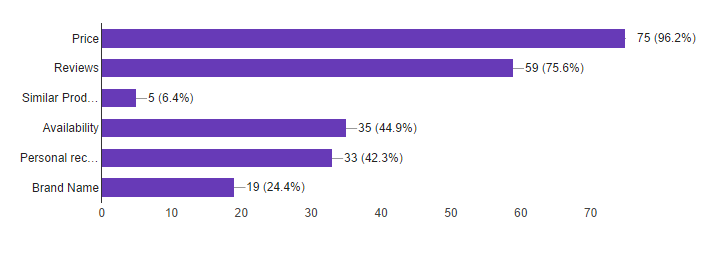
\includegraphics[width=0.9\columnwidth]{figures/ShoppingFactors}
	\caption{Phase One respondants identified price and reviews as the most critical factors in making their shopping decisions, while product comparisons---identified in later phases as ``highly useful''---were initially rated as least important. \textbf{DNS: Axis labels please!!! Also use full labels rather than ellipses. May have to reconstruct in powerpoint or inkscape}}
	\label{figures:ShoppingFactors}
\end{figure}

 \subsection{Methodology}
We conducted a preliminary survey across 78 participants over social media to identify important aspects of customers' in-store and online shopping experiences. We asked participants to respond to a series of open-ended and multiple selection questions to identify the three most important pieces of information involved their shopping decisions (Fig. \ref{figures:ShoppingFactors}), what they did and did not like about existing in-store and online shopping experiences, and ways they currently use mobile technology as part of their existing shopping experiences. 
%\todo{does this feel like a reasonable synopsis?}  \todo{JRB: Yes, except I would like to know if these were open-ended questions or not.}
We used the responses from our online survey to
%isolate -- JRB: WC?
identify 
factors of in-store and online shopping that were most important to our participants.  
% DNS: A lot of this was redundant with the sentence above, so have compacted to make space
%We also asked participants if they use a mobile device while in-store to make purchasing decisions.
%Figure \ref{figures:ShoppingFactors} details participants' responses when prompted for their three most important factors in making shopping decisions. Using open-ended questions, we asked participants what they liked the most and least about shopping online and in store. \

We clustered responses based on similarity and found that
%, resulting in the findings below.
%% JRB -- Removed, not needed: \subsection{Findings}
participants appreciate the immediacy and physical interaction with products in a store, but cited drawbacks included the inability to comparison shop, to get the lowest or most appropriate price,
% and/or feeling that they are paying too much, 
and store staff trying to influence purchase decisions.  Participants appreciate the ability to shop any time and from virtually any location
%freedom from store location and hours, 
\todo{I'm not sure what "freedom from store location and hours" means - EH} \todo{JRB: Ditto.} \todo{DNS: Is this a fair synopsis?} and low time-to-purchase of online shopping, \todo{I'm confused as to whether you're talking about things participants appreciate about in-store shopping or about online shopping. DNS: Took a pass at resolving. Does this align with what was intended?} but disliked the associated shipping charges and delivery wait times. 
% DNS: Removed as I'm not sure how this factors into the broader conclusions
%We also found that users are willing to spend more time researching more expensive products. 
These findings provided a foundation from which we engage in our design work in Phases Two and Three. \todo{DNS: Verify once this section is revised that it still sufficiently dovetails with the discussion section.}
